\documentclass[a4paper, 12pt]{article}

%=========
% PACKAGES
%=========

\usepackage{graphicx}
\usepackage[section]{placeins}
\usepackage{float}
\usepackage{amsmath}
\usepackage{listings}
\usepackage{xcolor}
\usepackage{extarrows}
\usepackage{verbatim}
\usepackage{enumerate}
\usepackage{enumitem}
\usepackage{eurosym}
\usepackage{svg}
\usepackage{varwidth}
\usepackage{moreverb}
\usepackage{relsize}
\usepackage{tabto}
\usepackage[margin=1in]{geometry}
\usepackage[normalem]{ulem}
\usepackage{units}
\usepackage{fancyvrb}
\usepackage{fontspec}
\usepackage{extarrows}
\usepackage{amsfonts}
\usepackage{amssymb}
\usepackage{hyperref}
%\usepackage{unicode-math}


%=====================
% SETTINGS/DEFINITIONS
%=====================

% Don't break words with hyphens. Instead, wrap word to next line.
\tolerance=1
% \emergencystretch=\maxdimen
\hyphenpenalty=10000
\hbadness=10000

\definecolor{codegreen}{rgb}{0,0.6,0}
\definecolor{codegray}{rgb}{0.5,0.5,0.5}
\definecolor{codepurple}{rgb}{0.58,0,0.82}
\definecolor{backcolour}{rgb}{0.95,0.95,0.92}

\def\verbatimtabsize{4}

\lstdefinestyle{mystyle}{
	backgroundcolor=\color{backcolour},
	commentstyle=\color{codegreen},
	keywordstyle=\color{magenta},
	numberstyle=\tiny\color{codegray},
	stringstyle=\color{codepurple},
	basicstyle=\ttfamily\footnotesize,
	breakatwhitespace=false,
	breaklines=true,
	captionpos=b,
	keepspaces=true,
	numbers=left,
	numbersep=5pt,
	showspaces=false,
	showstringspaces=false,
	showtabs=false,
	tabsize=2
}

\lstset{style=mystyle}

\setlength{\parindent}{0pt}
\setlength{\parskip}{0em}
\setlength{\jot}{4mm}

\pagenumbering{gobble}

\hypersetup{
    colorlinks=true,
    linkcolor=blue,
    filecolor=blue,      
    urlcolor=blue,
}

\setmainfont{Minion Pro}

\newcommand{\imagesPath}{results}
\newcommand{\myWidth}{0.8\linewidth}

\title{
	\textbf{Επεξεργασία Φωνής και Φυσικής Γλώσσας} \\~\\
	3η εργαστηριακή άσκηση
}

\author{
	Ηλίας Κουμουκέλης, el18157 \\
	Νικόλαος Παγώνας, el18175
}

\date{}

\begin{document}

\maketitle

\section*{Εισαγωγή}
    
    Σκοπός αυτής της εργαστηριακής άσκησης είναι να εμπλουτίσουμε την απλή αρχιτεκτονική της \\ προπαρασκευής με RNNs, Transfer Learning και attention mechanisms. Και πάλι χρησιμοποιούμε τα \verb|glove.6B.50d| embeddings, αλλά εδώ χρησιμοποιούμε μόνο το dataset \verb|MR|.

\section*{Ερώτημα 1}

    \subsection*{1.1}
    
        Πλέον υπολογίζουμε την αναπαράσταση κάθε πρότασης $u$ ως την συνένωση του μέσου όρου και του μεγίστου ανά διάσταση των embeddings της κάθε πρότασης $E=(e_1, e_2, \dots, e_N)$.
        
        \[
            u = \left[ mean(E) || max(E) \right]
        \]
        
    \subsection*{1.2}
    
        Με την συνεισφορά του μεγίστου (και όχι μόνο του μέσου όρου) μπορεί να δοθεί περισσότερη έμφαση σε ορισμένες λέξεις-κλειδιά, οι οποίες παίζουν σημαντικότερο ρόλο στην κατηγοριοποίηση με βάση το συναίσθημα. Αυτό είναι λογικό, αφού σε μία πρόταση οι περισσότερες λέξεις δεν αρκούν για να περιγράψουν αν το συναίσθημα της πρότασης είναι θετικό ή αρνητικό. Για παράδειγμα, οι προτάσεις:
        
        \begin{itemize}
            \item That was the \textbf{best} movie I have ever seen.
            \item That was the \textbf{worst} movie I have ever seen.
        \end{itemize}
        
        Διαφέρουν μόνο σε μία λέξη, ενώ οι υπόλοιπες 8 είναι ίδιες. Παρολαυτά, αυτή η μία λέξη διαφοροποιεί τις προτάσεις τόσο πολύ, που ουσιαστικά οι προτάσεις είναι άκρως αντίθετες σε συναίσθημα (πολύ θετικό έναντι πολύ αρνητικού). Μία ανάλυση που βασίζεται μόνο στον μέσο όρο θα μπορούσε να μειώσει την επίδραση που έχουν οι πολύ "φορτισμένες" λέξεις \verb|best| και \verb|worst|, ειδικά αν οι προτάσεις περιέχουν πολλές λέξεις. Με το max pooling όμως, οι σημαντικές λέξεις ξεχωρίζουν όπως πρέπει, ενώ ο συνδυασμός mean και max pooling αποτελεί μία μέση λύση, όπου οι λέξεις-κλειδιά ξεχωρίζουν μεν, αλλά δεν αναιρούν το νόημα όλης της υπόλοιπης πρότασης.
    
\section*{Ερώτημα 2}

    Σε αυτό το ερώτημα χρησιμοποιούμε ένα LSTM για την κωδικοποίηση της πρότασης, το οποίο θα διαβάζει τα word embeddings $e_i$ και θα παράγει μία νέα αναπαράσταση για κάθε λέξη $h_i$, η οποία θα λαμβάνει υπόψιν της και τα συμφραζόμενα.
    
    \subsection*{2.1}

        Εδώ χρησιμοποιούμε την τελευταία έξοδο του LSTM $h_N$ ως την αναπαράσταση του κειμένου $u$. Να σημειωθεί ότι χρησιμοποιούμε ως τελευταίο timestep το πραγματικό (εξαιρούμε δηλαδή το zero padding, όπως στην προπαρασκευή). Η υλοποίηση βρίσκεται στην κλάση \verb|Model21|, στο \verb|models.py|. \\
        
        Τα αποτελέσματα είναι τα εξής:
        
        \begin{itemize}
            \item Training dataset:
                \begin{itemize}
                    \item Accuracy: 0.828
                    \item Recall: 0.828
                    \item F1 Score: 0.827
                    \item Loss:
                        \begin{figure}[H]
                            \centering
                            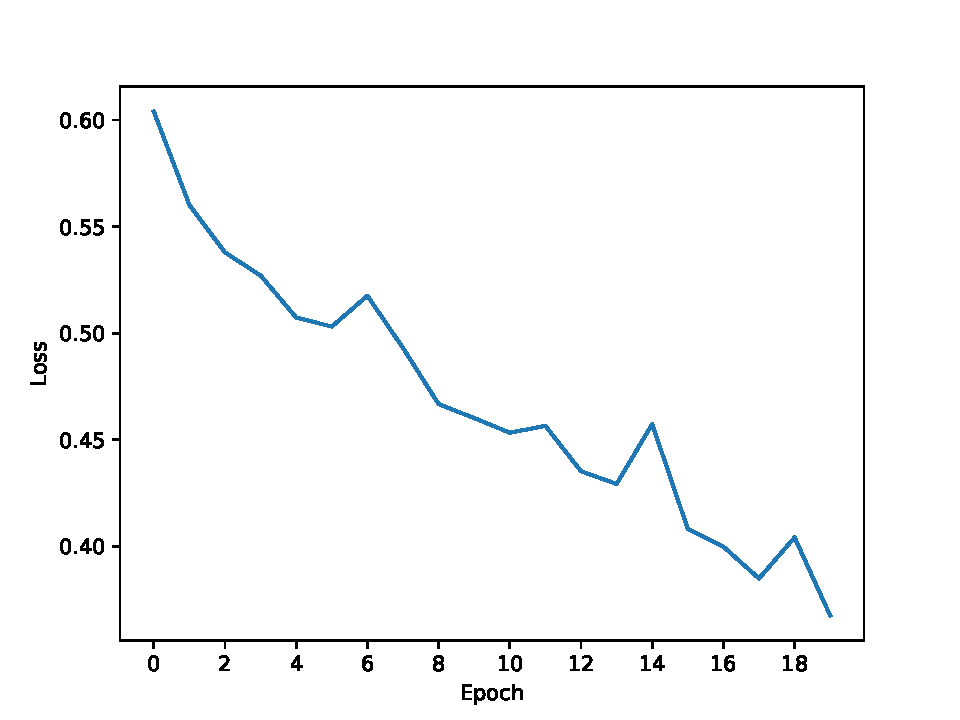
\includegraphics[width=\myWidth]{\imagesPath/Model21_train.pdf}
                        \end{figure}
                \end{itemize}
                
            \item Test dataset:
                \begin{itemize}
                    \item Accuracy: 0.769
                    \item Recall: 0.454
                    \item F1 Score: 0.496
                    \item Loss:
                        \begin{figure}[H]
                            \centering
                            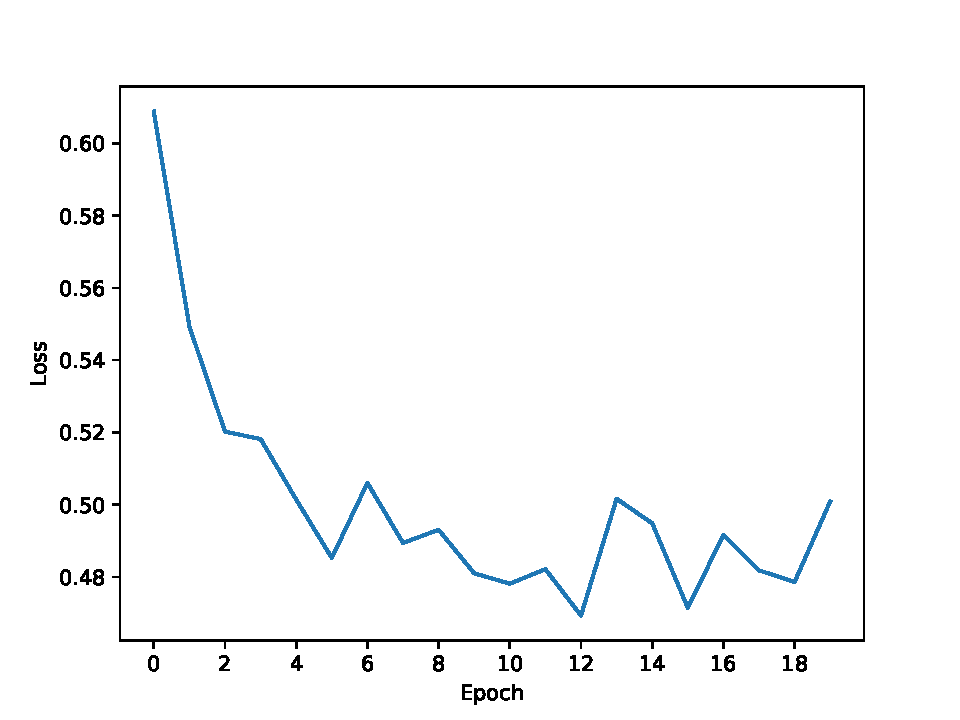
\includegraphics[width=\myWidth]{\imagesPath/Model21_test.pdf}
                        \end{figure}
                \end{itemize}
        \end{itemize}

    \subsection*{2.2} 
        
        Εδώ χρησιμοποιούμε ως αναπαράσταση του κειμένου $u$ την συνένωση:
        
        \[
            u = \left[ h_N || mean(E) || max(E) \right]
        \]
        
        Η υλοποίηση βρίσκεται στην κλάση \verb|Model22|, στο \verb|models.py|. \\
        
        Τα αποτελέσματα είναι τα εξής:
        
        \begin{itemize}
            \item Training dataset:
                \begin{itemize}
                    \item Accuracy: 0.840 
                    \item Recall: 0.839 
                    \item F1 score: 0.839 
                    \item Loss:
                        \begin{figure}[H]
                            \centering
                            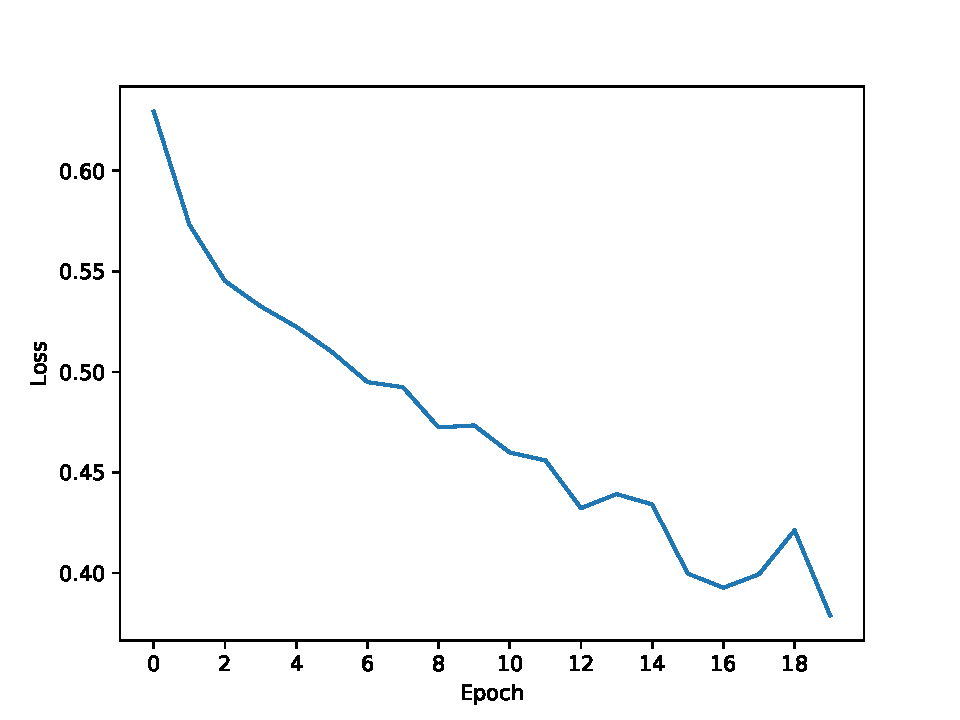
\includegraphics[width=\myWidth]{\imagesPath/Model22_train.pdf}
                        \end{figure}
                \end{itemize}
                
            \item Test dataset:
                \begin{itemize}
                    \item Accuracy: 0.778 
                    \item Recall: 0.482 
                    \item F1 score: 0.503 
                    \item Loss:
                        \begin{figure}[H]
                            \centering
                            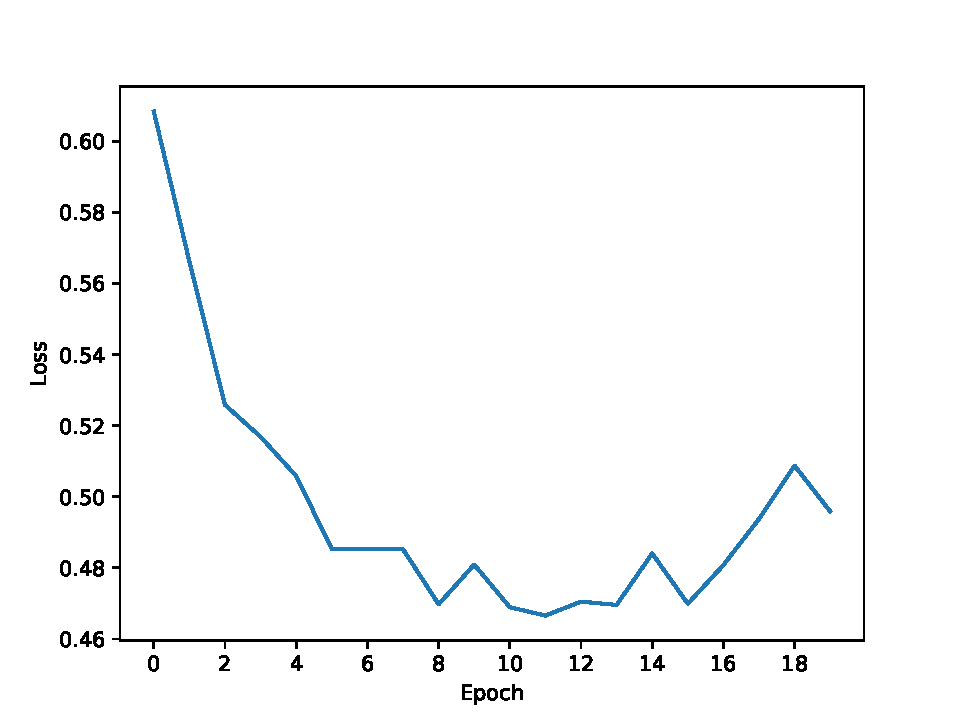
\includegraphics[width=\myWidth]{\imagesPath/Model22_test.pdf}
                        \end{figure}
                \end{itemize}
        \end{itemize}

\section*{Ερώτημα 3}
    
    Σε αυτό το ερώτημα χρησιμοποιούμε ένα μηχανισμό attention. Παίρνουμε έτοιμη την υλοποίηση που βρίσκεται \href{https://gist.github.com/cbaziotis/94e53bdd6e4852756e0395560ff38aa4}{σε αυτό το gist}.

    \subsection*{3.1}

        Χρησιμοποιούμε τον μηχανισμό attention, για να υπολογίσουμε την αναπαράσταση ενός κειμένου, ως το σταθμισμένο άθροισμα των word embeddings:
        
        \begin{align*}
            v_i &= tanh(We_i+b) \\
            a_i &= \dfrac{exp(v_i)}{\sum_{t=1}^{N}exp(u_t)}\\
            u   &= \sum_{i=1}^{N}a_ie_i\\
        \end{align*}
        
        Η υλοποίηση βρίσκεται στην κλάση \verb|Model31|, στο \verb|models.py|. \\
        
        Τα αποτελέσματα είναι τα εξής:
        
        \begin{itemize}
            \item Training dataset:
                \begin{itemize}
                    \item Accuracy: 0.726
                    \item Recall: 0.726
                    \item F1 Score: 0.724
                    \item Loss:
                        \begin{figure}[H]
                            \centering
                            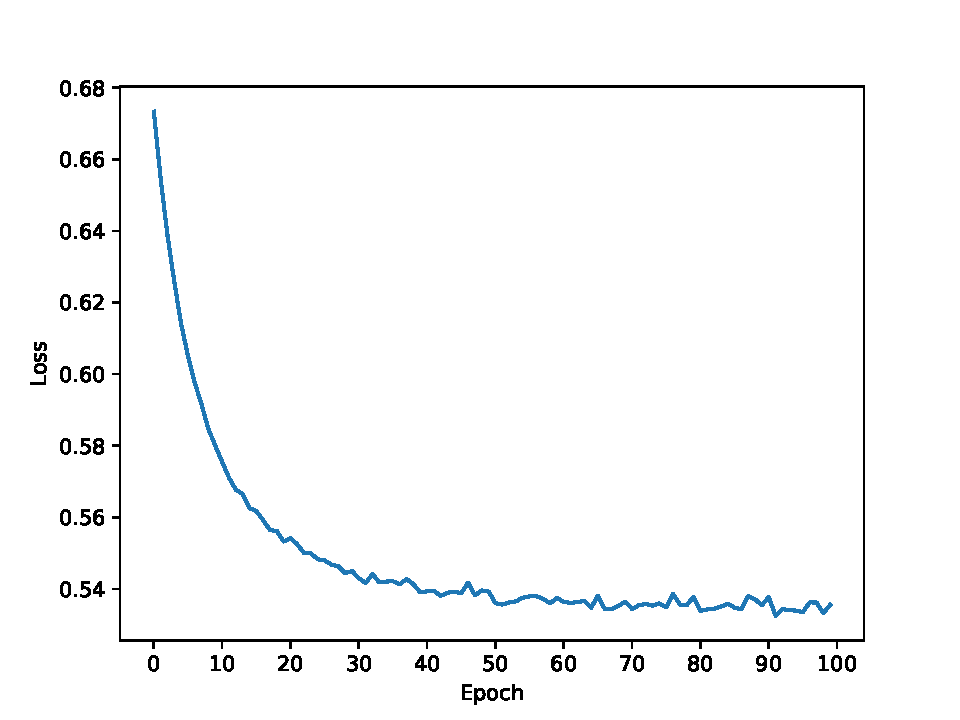
\includegraphics[width=\myWidth]{\imagesPath/Model31_train.pdf}
                        \end{figure}
                \end{itemize}
                
            \item Test dataset:
                \begin{itemize}
                    \item Accuracy: 0.734
                    \item Recall: 0.432
                    \item F1 Score: 0.478
                    \item Loss:
                        \begin{figure}[H]
                            \centering
                            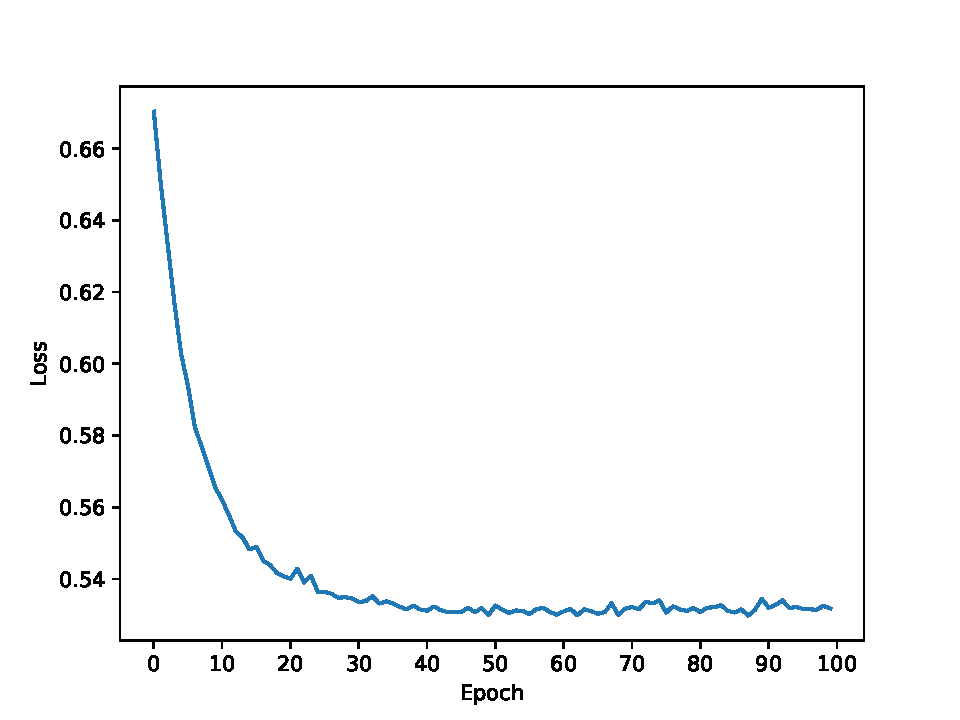
\includegraphics[width=\myWidth]{\imagesPath/Model31_test.pdf}
                        \end{figure}
                \end{itemize}
        \end{itemize}

    \subsection*{3.2}

        Πάλι χρησιμοποιούμε τον μηχανισμό attention για να υπολογίσουμε την αναπαράσταση ενός κειμένου, αλλά αυτή τη φορά ως το σταθμισμένο άθροισμα των εξόδων ενός LSTM.
        
        \begin{align*}
            v_i &= tanh(Wh_i+b) \\
            a_i &= \dfrac{exp(v_i)}{\sum_{t=1}^{N}exp(u_t)}\\
            u   &= \sum_{i=1}^{N}a_ih_i\\
        \end{align*}
        
        Η υλοποίηση βρίσκεται στην κλάση \verb|Model32|, στο \verb|models.py|. \\

        Τα αποτελέσματα είναι τα εξής:
        
        \begin{itemize}
            \item Training dataset:
                \begin{itemize}
                    \item Accuracy: 0.828
                    \item Recall: 0.828
                    \item F1 Score: 0.826
                    \item Loss:
                        \begin{figure}[H]
                            \centering
                            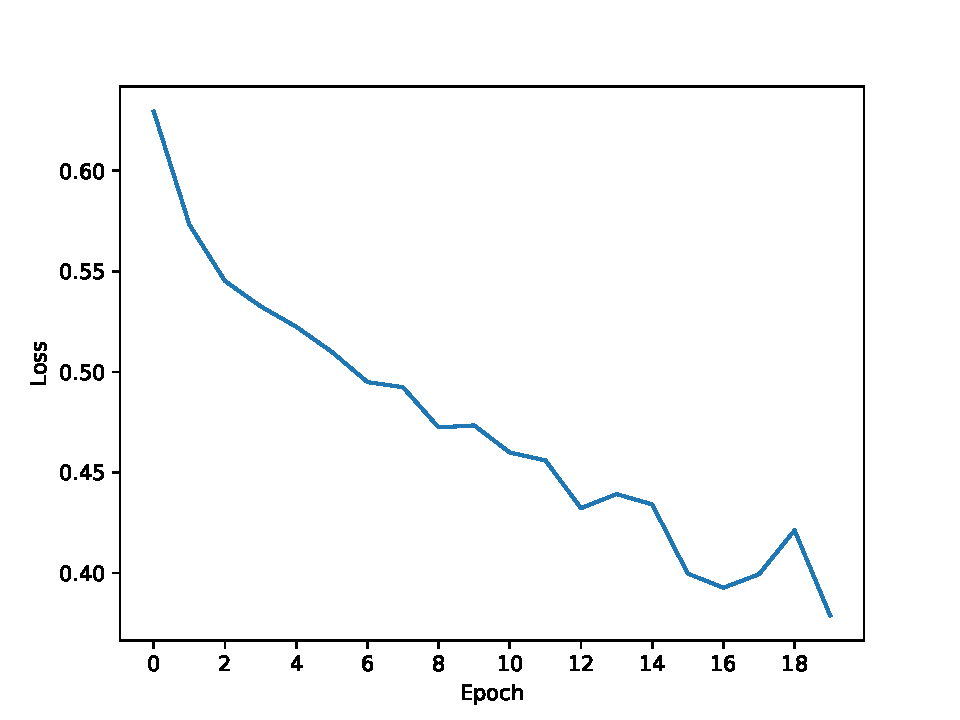
\includegraphics[width=\myWidth]{\imagesPath/Model32_train.pdf}
                        \end{figure}
                \end{itemize}
                
            \item Test dataset:
                \begin{itemize}
                    \item Accuracy: 0.745
                    \item Recall: 0.438
                    \item F1 Score: 0.485
                    \item Loss:
                        \begin{figure}[H]
                            \centering
                            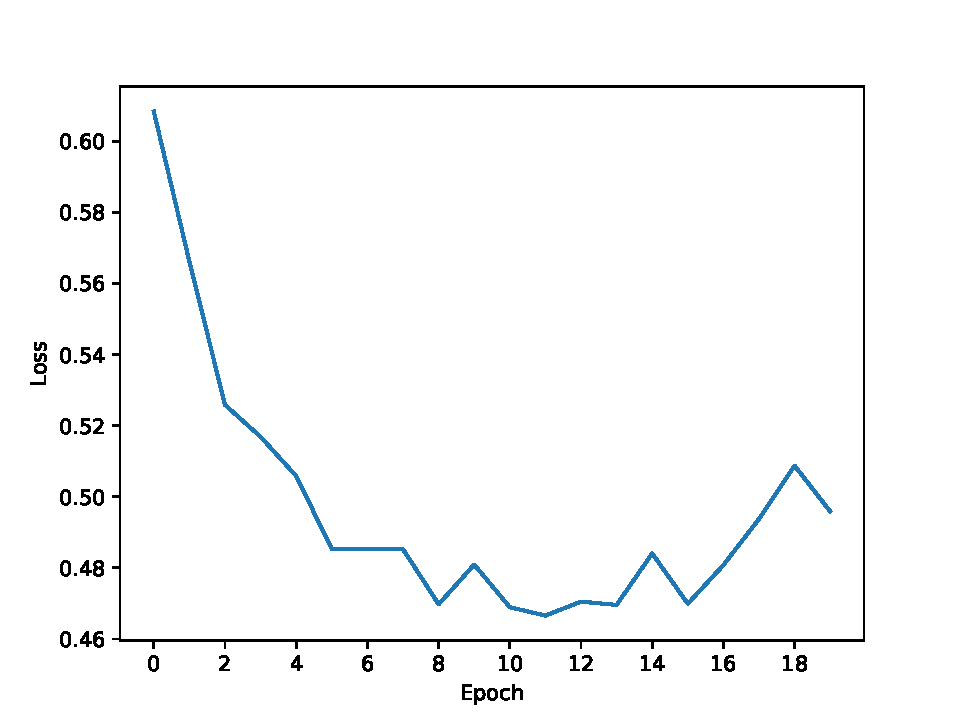
\includegraphics[width=\myWidth]{\imagesPath/Model32_test.pdf}
                        \end{figure}
                \end{itemize}
        \end{itemize}

\section*{Ερώτημα 4}
    
    Σε αυτό το ερώτημα υλοποιούμε τα ζητούμενα του ερωτήματος 3, αλλά αυτή τη φορά χρησιμοποιούμε ένα \textbf{αμφίδρομο} LSTM.  

    \subsection*{4.1} 

        Αυτό το ερώτημα είναι όμοιο με το 2.2, αλλά με αμφίδρομο LSTM. Η υλοποίηση βρίσκεται στην κλάση \verb|Model41|, στο \verb|models.py|. \\
        
        Τα αποτελέσματα είναι τα εξής:
        
        \begin{itemize}
            \item Training dataset:
                \begin{itemize}
                    \item Accuracy: 0.831 
                    \item Recall: 0.832 
                    \item F1 score: 0.828 
                    \item Loss:
                        \begin{figure}[H]
                            \centering
                            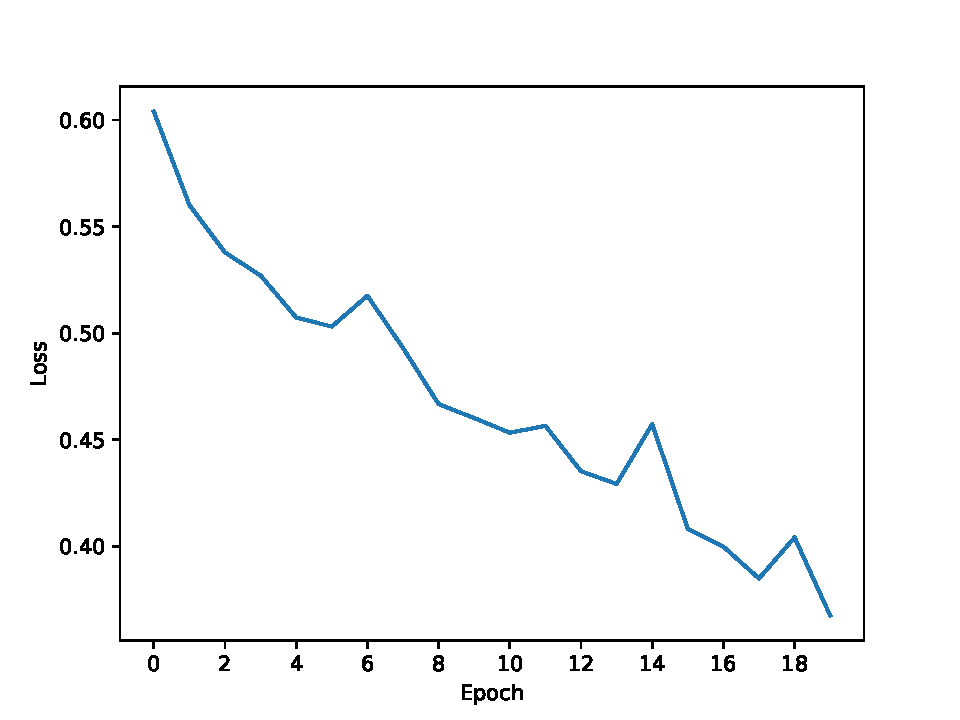
\includegraphics[width=\myWidth]{\imagesPath/Model41_train.pdf}
                        \end{figure}
                \end{itemize}
                
            \item Test dataset:
                \begin{itemize}
                    \item Accuracy: 0.782 
                    \item Recall: 0.523 
                    \item F1 score: 0.521 
                    \item Loss:
                        \begin{figure}[H]
                            \centering
                            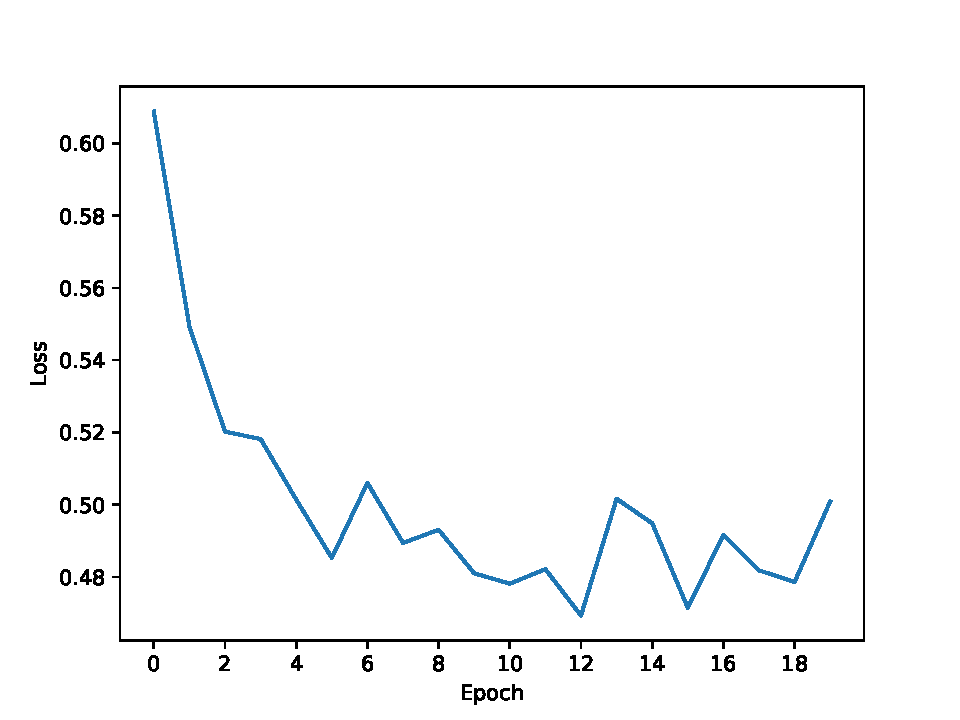
\includegraphics[width=\myWidth]{\imagesPath/Model41_test.pdf}
                        \end{figure}
                \end{itemize}
        \end{itemize}

    \subsection*{4.2}

        Αυτό το ερώτημα είναι όμοιο με το 3.2, αλλά με αμφίδρομο LSTM. Η υλοποίηση βρίσκεται στην κλάση \verb|Model42|, στο \verb|models.py|. \\
        
        Τα αποτελέσματα είναι τα εξής:
        
        \begin{itemize}
            \item Training dataset:
                \begin{itemize}
                    \item Accuracy: 0.821 
                    \item Recall: 0.819 
                    \item F1 score: 0.819 
                    \item Loss:
                        \begin{figure}[H]
                            \centering
                            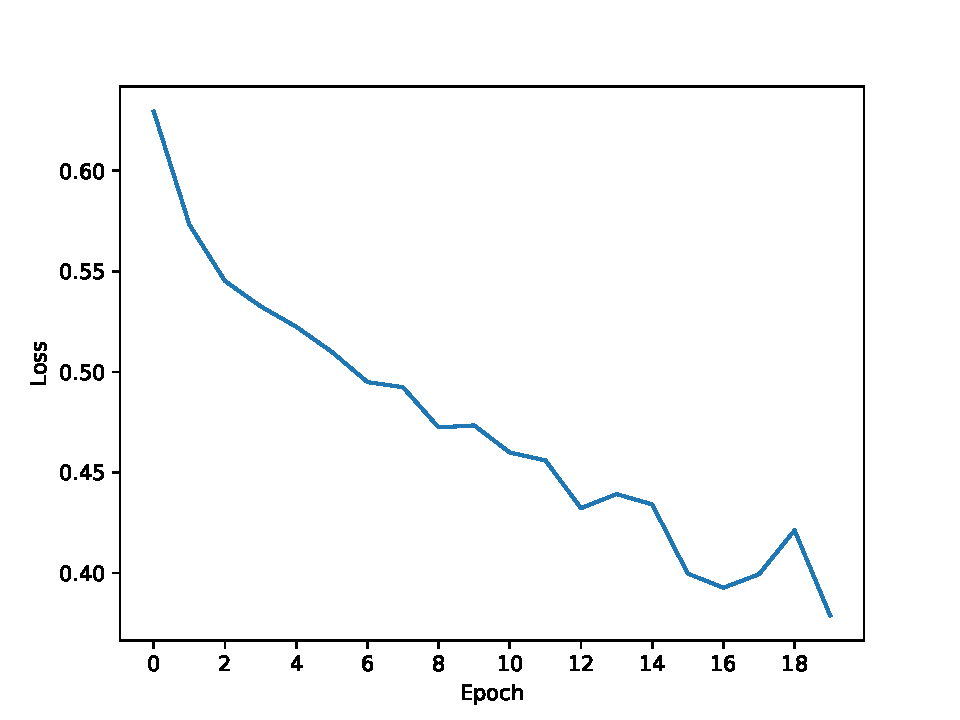
\includegraphics[width=\myWidth]{\imagesPath/Model42_train.pdf}
                        \end{figure}
                \end{itemize}
                
            \item Test dataset:
                \begin{itemize}
                    \item Accuracy: 0.790 
                    \item Recall: 0.781 
                    \item F1 score: 0.783
                    \item Loss:
                        \begin{figure}[H]
                            \centering
                            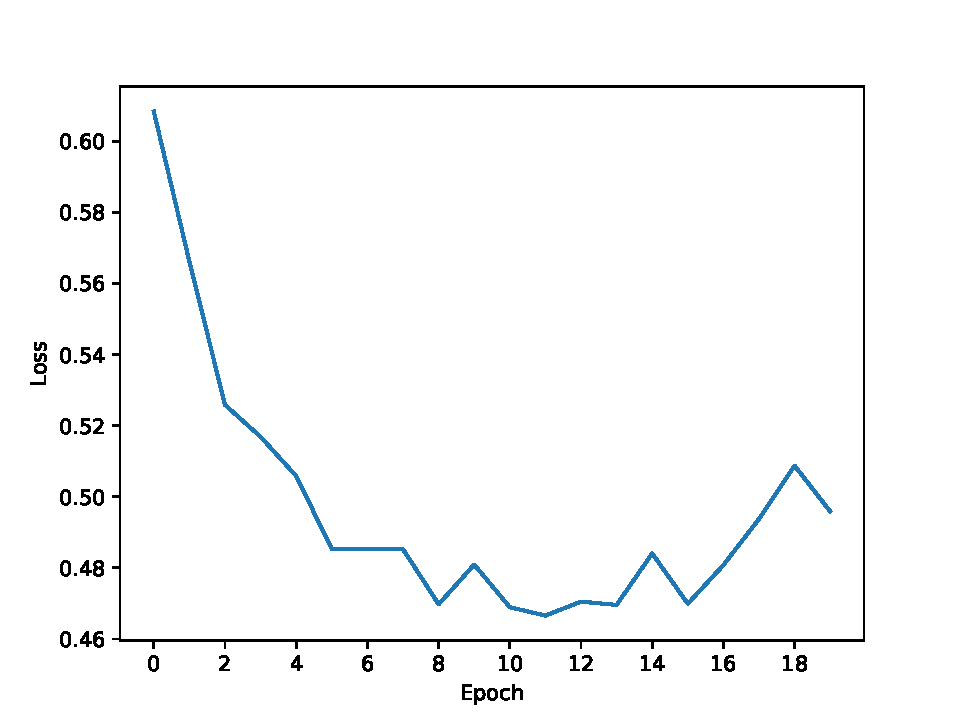
\includegraphics[width=\myWidth]{\imagesPath/Model42_test.pdf}
                        \end{figure}
                \end{itemize}
        \end{itemize}

\section*{Ερώτημα 5}

    \subsection*{5.1}

        ...

    \subsection*{5.2}

        ...

    \subsection*{5.3}

        ...

\section*{Ερώτημα 6}

    \subsection*{6.1}
        
        ...
    
    \subsection*{6.2}
        
        Τα BoW χαρακτηριστικά θα μπορούσουν να οδηγήσουν σε καλύτερα αποτελέσματα σε σχέση με αναπαραστάσεις όπως ο μέσος όρος των word embeddings, σε περιπτώσεις όπου:
        
        \begin{itemize}
            \item Θέλουμε να δημιουργήσουμε baseline models, αφού πολύ εύκολα και γρήγορα, με έτοιμες \\ συναρτήσεις βιβλιοθηκών, και χωρίς περίπλοκες αναπαραστάσεις, μπορούμε να φτιάξουμε μία απλοϊκή μορφή μοντέλων για κατηγοριοποίηση κειμένων.
            \item Το dataset είναι μικρό σε μέγεθος και έχουμε να κάνουμε με domain-specific context. Όταν τα κείμενα περιέχουν εξειδικευμένους/τεχνικούς όρους, τα pretrained embeddings που υπάρχουν δεν αποδίδουν τόσο καλά, γιατί είναι πολύ γενικά, και ταυτόχρονα είναι πιο δύσκολο να βρούμε τόσο εξειδικευμένα pretrained embeddings. Έτσι, προτιμάται η αναπαράσταση με \\ χαρακτηριστικά tfidf.
        \end{itemize}
\end{document}